\clearpage
\subsection{Decoding the winning block back to a formula}
A low Ising energy becomes a material recommendation only after the binary state has been decoded and compared across blocks. Figure~\ref{fig:decode} follows the Q3 winner. Holding Sn and Ti fixed, the three family scores are 3.2681 for O3, 8.2041 for FO2 and 12.3445 for NO2. The envelope stores the first value together with the O3 family and original row ID 8760.

\begin{figure}[ht]
\centering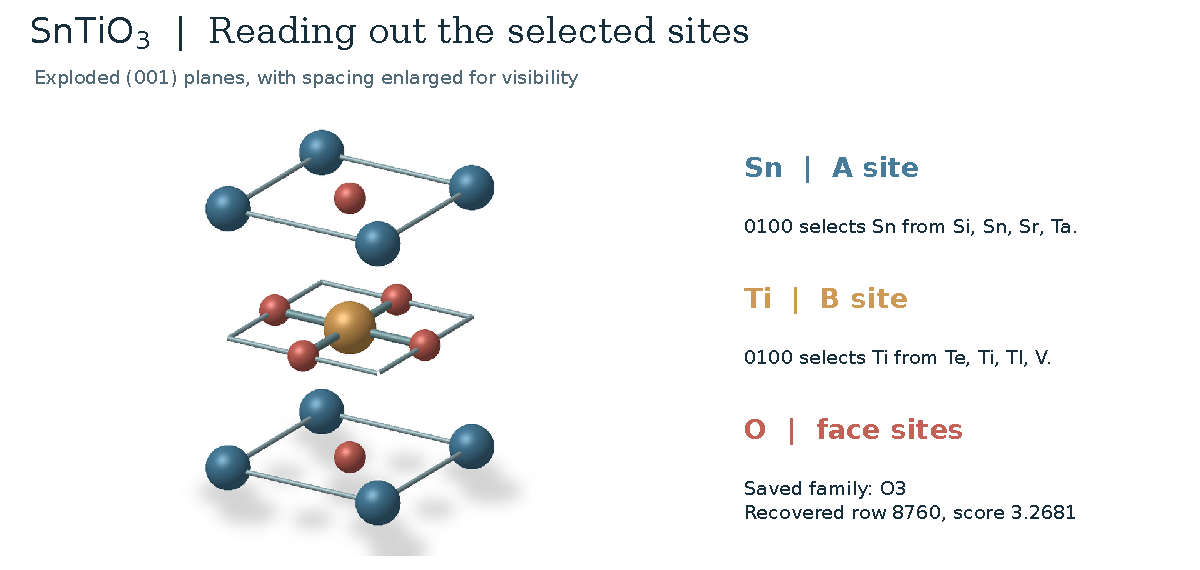
\includegraphics[width=\linewidth]{figures/qubo_decode.pdf}
\caption{Exploded view of the decoded Q3 winner. The blue Sn atoms occupy A sites, the gold Ti atom occupies the central B site, and the saved O3 family fills the face sites. Two boundary SnO planes surround a TiO$_2$ plane. Periodic sharing gives one SnTiO$_3$ formula unit. Vertical spacing is expanded for visibility.}\label{fig:decode}
\end{figure}

The maximum cost in this block is 38.222147. Scaling the selected score by $15/M$ gives 1.283 to three decimals, which rounds to one. The ordering $(\mathrm{Si,Sn,Sr,Ta})$ on A and $(\mathrm{Te,Ti,Tl,V})$ on B makes the second bit active in each register. If $\sigma_i$ is a returned spin and $\sigma_r$ the reference spin, the implemented readout is
\[
 z_i=\tfrac12(1+\sigma_i\sigma_r).
\]
Simultaneously reversing every spin leaves every product unchanged. The two gauge representations therefore identify the same pair and should be counted once. Fixing the reference to $+1$ gives binary vectors $(0,1,0,0)$ on both sides. The winning state's measured SDK energy is $-724$ and the decoded raw score is 3.268113. The block's lowest integer cost has one legal pair. Other blocks have different scale factors and omitted constants; their winners enter the final comparison through their raw scores.

\subhead{Why use four elements on each side?}
For a block of $n$ rows and $n$ columns with integer costs in $[0,K]$, the reference coupling of one logical variable has magnitude bounded by
\[
 B(n,K,P)=2P(n-2)+nK,\qquad n\geq2 .
\]
The $n-1$ same-register partners each contribute $2P$ and the diagonal contributes $-2P$ inside the reference term. Each of the $n$ cross-register partners contributes at most $K$. With $P=16$, $K=15$, blocks of side three, four and five have respective bounds 77, 124 and 171. Four is the largest uniform side length guaranteed to fit signed eight-bit couplings under this integer scaling. A particular five-element block may fit if its row and column sums are small. The uniform construction eliminates that data-dependent assumption.

